\documentclass[12pt,a4paper]{article}

% ─── Page Layout ───────────────────────────────────────────────────────────────
\usepackage[a4paper, margin=0.8in, headheight=14pt]{geometry}

% ─── Fonts (XeLaTeX) ───────────────────────────────────────────────────────────
\usepackage{fontspec}
\usepackage{unicode-math}
\setmainfont{TeX Gyre Pagella}
\setmonofont[Scale=0.88]{TeX Gyre Cursor}
\setmathfont{Latin Modern Math}

% ─── Packages ──────────────────────────────────────────────────────────────────
\usepackage{xcolor}
\usepackage{colortbl}
\usepackage{titlesec}
\usepackage{enumitem}
\usepackage{tabularx}
\usepackage{booktabs}
\usepackage{array}
\usepackage{amsmath}
\usepackage{tikz}
\usetikzlibrary{shapes.geometric, arrows.meta, positioning, calc, fit, decorations.pathreplacing}
\usepackage{tcolorbox}
\tcbuselibrary{skins, breakable}
\usepackage{hyperref}
\usepackage{fancyhdr}
\usepackage{graphicx}
\usepackage{microtype}
\hyphenpenalty=10000
\exhyphenpenalty=10000
\sloppy
\usepackage{caption}
\usepackage{setspace}
\usepackage{multirow}
\usepackage{tocloft}

% ─── Q&A helper ────────────────────────────────────────────────────────────────
\newcommand{\Q}[1]{\textbf{#1}\par\noindent\ignorespaces}

% ─── Colour Palette ────────────────────────────────────────────────────────────
\definecolor{myred}{RGB}{196,30,58}
\definecolor{mydark}{RGB}{30,30,50}
\definecolor{mygreen}{RGB}{14,120,80}
\definecolor{myteal}{RGB}{0,130,140}
\definecolor{myamber}{RGB}{180,100,0}
\definecolor{mypurple}{RGB}{100,30,160}
\definecolor{mygray}{RGB}{246,247,249}
\definecolor{mgframe}{RGB}{180,185,200}
\definecolor{watermark}{RGB}{145,150,170}
\definecolor{hdrred}{RGB}{250,232,235}
\definecolor{hdrgreen}{RGB}{220,244,233}
\definecolor{hdrteal}{RGB}{220,242,244}
\definecolor{hdramber}{RGB}{253,242,215}
\definecolor{hdrpurple}{RGB}{238,228,255}
\definecolor{hdrgray}{RGB}{238,240,245}
\definecolor{rowalt}{RGB}{250,251,253}

% ─── Section Formatting ────────────────────────────────────────────────────────
\titleformat{\section}
  {\large\bfseries\color{myred}}{\thesection.}{0.5em}{}
  [\vspace{1pt}{\color{myred}\rule{\linewidth}{0.8pt}}]
\titleformat{\subsection}
  {\normalsize\bfseries\color{myteal}}{\thesubsection}{0.5em}{}
\titlespacing*{\section}{0pt}{18pt}{7pt}
\titlespacing*{\subsection}{0pt}{11pt}{4pt}

% ─── Paragraph ─────────────────────────────────────────────────────────────────
\setlength{\parindent}{0pt}
\setlength{\parskip}{4pt}

% ─── TOC Styling ───────────────────────────────────────────────────────────────
\renewcommand{\cfttoctitlefont}{\large\bfseries\color{myred}}
\renewcommand{\cftaftertoctitle}{\par\noindent{\color{myred}\rule{\linewidth}{0.8pt}}}
\setlength{\cftbeforetoctitleskip}{0pt}
\setlength{\cftaftertoctitleskip}{6pt}
\renewcommand{\cftsecfont}{\normalsize\bfseries\color{mydark}}
\renewcommand{\cftsecpagefont}{\normalsize\bfseries\color{mydark}}
\renewcommand{\cftsecleader}{\cftdotfill{\cftdotsep}}
\setlength{\cftbeforesecskip}{7pt}
\renewcommand{\cftsubsecfont}{\small\color{mydark}}
\renewcommand{\cftsubsecpagefont}{\small\color{mydark}}
\setlength{\cftbeforesubsecskip}{3pt}
\setlength{\cftsubsecindent}{1.4em}

% ─── Table helpers ─────────────────────────────────────────────────────────────
\renewcommand{\arraystretch}{1.45}
\setlength{\tabcolsep}{6pt}
\arrayrulecolor{mydark}
\newcolumntype{B}[1]{>{\small\bfseries\raggedright\arraybackslash}m{#1}}
\newcolumntype{Y}{>{\small\raggedright\arraybackslash}X}
\renewcommand{\tabularxcolumn}[1]{m{#1}}

% ─── Header / Footer ───────────────────────────────────────────────────────────
\pagestyle{fancy}
\fancyhf{}
\fancyhead[L]{\small\color{myred}\textbf{PE-EC603C}\;\color{mydark}--- CMOS VLSI Design}
\fancyhead[R]{\small\color{myteal}\textbf{Module 1 Notes}}
\fancyfoot[C]{\small\color{mydark}\thepage}
\fancyfoot[R]{\small\color{watermark}\textit{\copyright\ Biraj}}
\renewcommand{\headrulewidth}{0.5pt}
\renewcommand{\footrulewidth}{0.3pt}

% ─── Hyperref ──────────────────────────────────────────────────────────────────
\hypersetup{
  colorlinks=true, linkcolor=myteal, urlcolor=myteal,
  pdfauthor={Biraj Sarkar},
  pdftitle={PE-EC603C --- Module 1 Notes}
}

% ─── tcolorbox styles ──────────────────────────────────────────────────────────
\tcbset{
  tikzbox/.style={
    colback=mygray, colframe=mgframe, boxrule=0.6pt, arc=4pt,
    left=8pt, right=8pt, top=6pt, bottom=6pt,
    colbacktitle=mgframe, coltitle=mydark,
    fonttitle=\small\bfseries
  },
  defbox/.style={
    colback=hdrgreen, colframe=mygreen, boxrule=0.8pt, arc=4pt,
    left=9pt, right=9pt, top=6pt, bottom=6pt,
    colbacktitle=mygreen, coltitle=white,
    fonttitle=\small\bfseries
  },
  formulabox/.style={
    colback=hdrteal, colframe=myteal, boxrule=0.8pt, arc=4pt,
    left=9pt, right=9pt, top=7pt, bottom=7pt,
    colbacktitle=myteal, coltitle=white,
    fonttitle=\small\bfseries
  },
  examplebox/.style={
    colback=hdramber, colframe=myamber, boxrule=0.8pt, arc=4pt,
    left=9pt, right=9pt, top=6pt, bottom=6pt,
    colbacktitle=myamber, coltitle=white,
    fonttitle=\small\bfseries
  },
  masonbox/.style={
    colback=hdrpurple, colframe=mypurple, boxrule=0.8pt, arc=4pt,
    left=9pt, right=9pt, top=6pt, bottom=6pt,
    colbacktitle=mypurple, coltitle=white,
    fonttitle=\small\bfseries
  },
  exambox/.style={
    colback=hdrpurple, colframe=mypurple, boxrule=1pt, arc=5pt,
    left=10pt, right=10pt, top=8pt, bottom=8pt,
    colbacktitle=mypurple, coltitle=white,
    fonttitle=\bfseries,
    breakable, title after break={\textbf{Frequently Asked / Viva Questions (contd.)}}}
}
% Make all boxes breakable across pages
\tcbset{breakable}

% ─── TikZ styles ───────────────────────────────────────────────────────────────
\tikzset{
  block/.style={rectangle, draw=myteal, fill=hdrteal,
    text width=2.4cm, align=center, minimum height=0.95cm,
    font=\small, rounded corners=3pt, line width=0.7pt},
  redblock/.style={rectangle, draw=myred, fill=hdrred,
    text width=2.4cm, align=center, minimum height=0.95cm,
    font=\small, rounded corners=3pt, line width=0.7pt},
  greenblock/.style={rectangle, draw=mygreen, fill=hdrgreen,
    text width=2.4cm, align=center, minimum height=0.95cm,
    font=\small, rounded corners=3pt, line width=0.7pt},
  amberblock/.style={rectangle, draw=myamber, fill=hdramber,
    text width=2.4cm, align=center, minimum height=0.95cm,
    font=\small, rounded corners=3pt, line width=0.7pt},
  purpblock/.style={rectangle, draw=mypurple, fill=hdrpurple,
    text width=2.4cm, align=center, minimum height=0.95cm,
    font=\small, rounded corners=3pt, line width=0.7pt},
  sumjunc/.style={circle, draw=myamber, fill=hdramber,
    minimum size=0.62cm, font=\small, line width=0.8pt},
  arrow/.style={-Stealth, thick, color=mydark},
  redarrow/.style={-Stealth, thick, color=myred},
  line/.style={thick, color=mydark}
}

% ═══════════════════════════════════════════════════════════════════════════════
\begin{document}
% ═══════════════════════════════════════════════════════════════════════════════

\begin{center}
  {\LARGE\bfseries\color{myred} PE-EC603C --- CMOS VLSI Design}\\[5pt]
  {\normalsize\color{mydark} Semester VI \quad$\bullet$\quad 3L:0T:0P \quad$\bullet$\quad 3 Credits}\\[3pt]
  {\normalsize\color{myteal}\textbf{Module 1 Exam Notes: VLSI Design Flow \& MOSFET Physics}}\\[3pt]
  {\small\color{mydark} CGEC \;$|$\; B.Tech ECE (2023--27) \;$|$\; \textit{Biraj Sarkar}}
\end{center}
\vspace{2pt}
\noindent{\color{myred}\rule{\linewidth}{1.5pt}}
\vspace{2pt}

\hypersetup{linkcolor=mydark}
\tableofcontents
\hypersetup{linkcolor=myteal}
\newpage

% ===============================================================================
\section{VLSI Design Methodologies}
% ===============================================================================

Very Large Scale Integration (VLSI) is the process of creating an integrated circuit (IC) by combining millions of MOS transistors onto a single silicon chip.

\subsection{Moore's Law}
Coined by Gordon Moore in 1965, it is an empirical observation that has driven the semiconductor industry.

\begin{tcolorbox}[defbox, title={\textbf{Moore's Law Statement}}]
The number of transistors on a microchip doubles approximately every two years, while the cost of computers is halved.
\end{tcolorbox}
\begin{itemize}[leftmargin=*, itemsep=3.5pt]
  \item \textbf{Significance}: Guided strategic planning, driven exponential scaling of speed/memory, and decreased cost-per-transistor.
  \item \textbf{Limits to Scaling}: High power density (thermal limits), subthreshold leakage, and quantum tunneling (as oxide thickness drops below $1\,\text{nm}$).
\end{itemize}

\subsection{VLSI Design Flow (Gajski-Yuhan Y-Chart)}
The Y-Chart characterizes the design flow along three different domains of representation (axes) radiating from a central point:
\begin{enumerate}[label=\arabic*., leftmargin=*]
  \item \textbf{Behavioral Domain (Abstraction):} Describes what the system does (algorithms, RTL, transfer functions).
  \item \textbf{Structural Domain (Interconnectivity):} Describes how components connect (CPUs, ALUs, logic gates, transistors).
  \item \textbf{Physical/Geometric Domain (Layout):} Describes where components are physically placed on silicon (floorplans, cells, layout masks).
\end{enumerate}

\begin{tcolorbox}[tikzbox, title={Gajski-Yuhan Y-Chart Design Flow}]
\centering
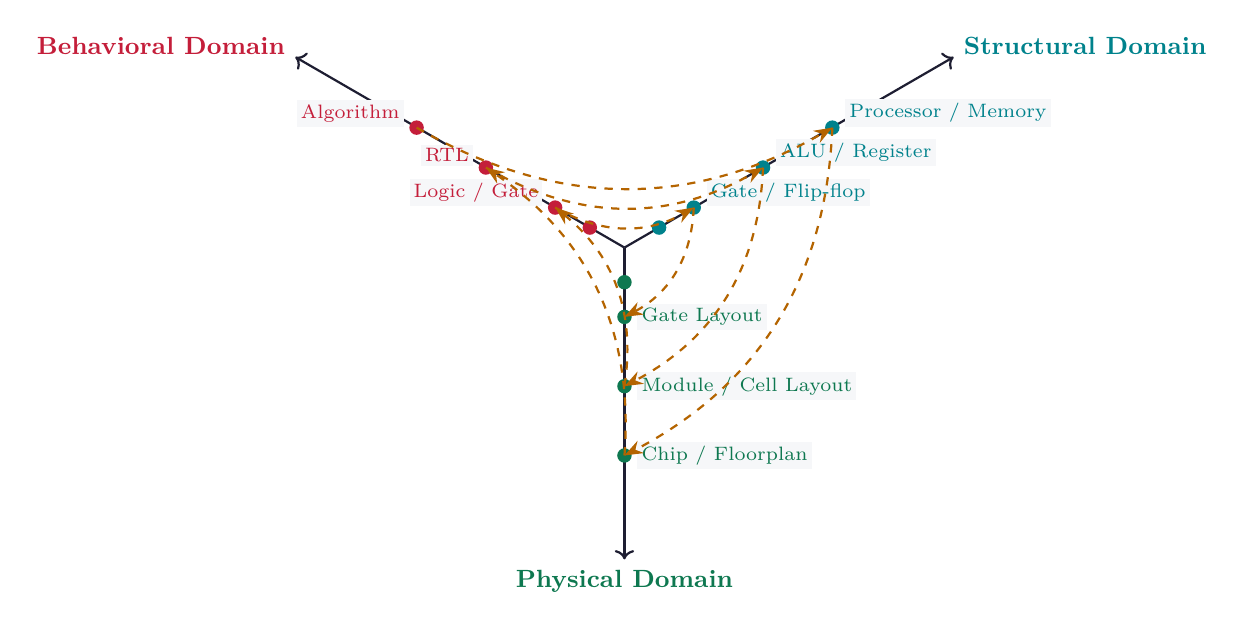
\begin{tikzpicture}[scale=1.1, thick, font=\small]
  % Draw three axes radiating from center (extended to prevent text collision)
  \draw[line, ->] (0, 0) -- (-3.8, 2.2) node[above left, color=myred, yshift=-0.1cm] {\textbf{Behavioral Domain}};
  \draw[line, ->] (0, 0) -- (3.8, 2.2) node[above right, color=myteal, yshift=-0.1cm] {\textbf{Structural Domain}};
  \draw[line, ->] (0, 0) -- (0, -3.6) node[below, color=mygreen] {\textbf{Physical Domain}};

  % Abstraction levels markers (Behavioral) - shifted and styled with background fill to prevent curve collision
  \filldraw[myred] (-2.4, 1.385) circle (2pt) node[above left, font=\scriptsize, fill=mygray, inner sep=1.5pt, xshift=-0.15cm] {Algorithm};
  \filldraw[myred] (-1.6, 0.924) circle (2pt) node[above left, font=\scriptsize, fill=mygray, inner sep=1.5pt, xshift=-0.15cm] {RTL};
  \filldraw[myred] (-0.8, 0.462) circle (2pt) node[above left, font=\scriptsize, fill=mygray, inner sep=1.5pt, xshift=-0.15cm] {Logic / Gate};
  \filldraw[myred] (-0.4, 0.231) circle (2pt);

  % Abstraction levels markers (Structural) - shifted and styled with background fill to prevent curve collision
  \filldraw[myteal] (2.4, 1.385) circle (2pt) node[above right, font=\scriptsize, fill=mygray, inner sep=1.5pt, xshift=0.15cm] {Processor / Memory};
  \filldraw[myteal] (1.6, 0.924) circle (2pt) node[above right, font=\scriptsize, fill=mygray, inner sep=1.5pt, xshift=0.15cm] {ALU / Register};
  \filldraw[myteal] (0.8, 0.462) circle (2pt) node[above right, font=\scriptsize, fill=mygray, inner sep=1.5pt, xshift=0.15cm] {Gate / Flip-flop};
  \filldraw[myteal] (0.4, 0.231) circle (2pt);

  % Abstraction levels markers (Physical) - shifted and styled with background fill to prevent curve collision
  \filldraw[mygreen] (0, -2.4) circle (2pt) node[right, font=\scriptsize, fill=mygray, inner sep=1.5pt, xshift=0.15cm] {Chip / Floorplan};
  \filldraw[mygreen] (0, -1.6) circle (2pt) node[right, font=\scriptsize, fill=mygray, inner sep=1.5pt, xshift=0.15cm] {Module / Cell Layout};
  \filldraw[mygreen] (0, -0.8) circle (2pt) node[right, font=\scriptsize, fill=mygray, inner sep=1.5pt, xshift=0.15cm] {Gate Layout};
  \filldraw[mygreen] (0, -0.4) circle (2pt);

  % Draw synthesis spirals/arrows showing mapping from behavioral to structural to physical
  \draw[arrow, color=myamber, bend right=30, dashed] (-2.4, 1.385) to (2.4, 1.385);
  \draw[arrow, color=myamber, bend left=30, dashed] (2.4, 1.385) to (0, -2.4);
  
  \draw[arrow, color=myamber, bend right=30, dashed] (0, -2.4) to (-1.6, 0.924);
  \draw[arrow, color=myamber, bend right=30, dashed] (-1.6, 0.924) to (1.6, 0.924);
  \draw[arrow, color=myamber, bend left=30, dashed] (1.6, 0.924) to (0, -1.6);
  
  \draw[arrow, color=myamber, bend right=30, dashed] (0, -1.6) to (-0.8, 0.462);
  \draw[arrow, color=myamber, bend right=30, dashed] (-0.8, 0.462) to (0.8, 0.462);
  \draw[arrow, color=myamber, bend left=30, dashed] (0.8, 0.462) to (0, -0.8);
\end{tikzpicture}
\end{tcolorbox}

\subsection{Design Hierarchy (Top-Down vs. Bottom-Up)}
\begin{itemize}[leftmargin=*, itemsep=3.5pt]
  \item \textbf{Top-Down Design Flow}: Starts at the system level (behavioral description) and recursively decomposes the system into functional blocks down to logic gates and transistor layouts. Highly automated and preferred for complex VLSI chips.
  \item \textbf{Bottom-Up Design Flow}: Starts at the lowest transistor level, building basic library cells (NAND, Flip-Flops) and grouping them into larger blocks until the system-level chip is constructed. Used for custom analog blocks and layout optimizations.
\end{itemize}

\section{VLSI Design Styles}

\subsection{Full Custom Design}
Every transistor, wire, and layer is custom-designed manually.
\begin{itemize}[leftmargin=*, itemsep=3.5pt]
  \item \textbf{Features}: Yields the highest possible performance, smallest silicon area, and lowest power dissipation.
  \item \textbf{Drawbacks}: Extremely high engineering cost, very long design cycle (time-to-market), and high risk of errors. Reserved for high-volume processors and analog blocks.
\end{itemize}

\subsection{Semi-Custom Design}
\begin{itemize}[leftmargin=*, itemsep=3.5pt]
  \item \textbf{Standard-Cell Based Design:} Layout is composed of pre-designed, pre-tested cell libraries (AND, flip-flops) placed in rows. Wires are routed automatically in channels between cell rows. Offers a balance between performance, design time, and cost.
  \item \textbf{Gate Array Based Design:} Wafers containing regular arrays of uncommitted transistors are pre-fabricated up to the metal contact level. Design customization is done only on the final metal interconnect mask layers. Very fast turnaround time and low mask cost, but lower utilization and speed.
  \item \textbf{FPGA (Field Programmable Gate Array):} Contains pre-fabricated programmable logic blocks (LUTs) and routing matrices. Configured electrically by loading configuration bits (RAM/Flash) without mask fabrication. Zero mask cost, instant turnaround, but has higher area and lower speed compared to ASICs.
\end{itemize}

\begin{tcolorbox}[tikzbox, title={Comparison of Design Methodologies}]
\renewcommand{\arraystretch}{1.4}
\par\noindent
\begin{tabularx}{\linewidth}{|B{2.2cm}|Y|Y|Y|}
\hline
\textbf{Feature} & \textbf{\color{myred}Full Custom} & \textbf{\color{myteal}Standard-Cell} & \textbf{\color{myamber}FPGA} \\
\hline
\textbf{Design Time} & Very Long (Months/Years) & Medium (Weeks/Months) & Very Short (Hours/Days) \\
\hline
\textbf{NRE Mask Cost} & Extremely High & High & Zero \\
\hline
\textbf{Performance} & Maximum & High & Moderate \\
\hline
\textbf{Unit Cost} & Low (at high volume) & Medium & High (due to overhead) \\
\hline
\textbf{Flexibility} & Zero (after tape-out) & Zero (after tape-out) & Re-programmable \\
\hline
\end{tabularx}
\end{tcolorbox}

\newpage
% ===============================================================================
\section{MOSFET Physical Operation}
% ===============================================================================

An n-channel MOSFET consists of a p-type silicon substrate (body), two heavily doped n+ regions (source and drain), and a metal/polysilicon gate insulated from the substrate by a thin silicon dioxide ($\text{SiO}_2$) layer.

\subsection{MOS Capacitor Operating Regions}
With the source and body grounded ($V_S = V_B = 0\,\text{V}$), as the gate voltage $V_G$ increases:
\begin{enumerate}[label=\alph*., leftmargin=*]
  \item \textbf{Accumulation ($V_G < V_{FB}$):} Negative charge on the gate attracts majority holes from the p-substrate to the silicon-oxide interface.
  \item \textbf{Depletion ($V_{FB} < V_G < V_{th}$):} Small positive gate voltage repels holes away from the interface, leaving behind fixed, negative acceptor ions ($N_A^-$), forming a carrier-free depletion region.
  \item \textbf{Inversion ($V_G > V_{th}$):} A large positive gate voltage bends the energy bands down sufficiently to attract minority electrons from the substrate and n+ source/drain to the interface. This forms a thin, conducting n-channel directly beneath the oxide.
\end{enumerate}

\subsection{Threshold Voltage ($V_{th}$)}
The threshold voltage is the minimum gate-to-source voltage required to induce strong inversion (creation of the conducting channel).

\begin{tcolorbox}[formulabox, title={\textbf{Threshold Voltage Formula}}]
For a p-substrate device:
\begin{equation}
  V_{th} = \Phi_{MS} + 2\phi_F - \frac{Q_{ox}}{C_{ox}} - \frac{Q_d}{C_{ox}}
\end{equation}
where:
\begin{itemize}[leftmargin=*, itemsep=2pt, topsep=2pt]
  \item $\Phi_{MS}$: Metal-semiconductor work function difference.
  \item $\phi_F$: Bulk Fermi potential: $\phi_F = V_T \ln(N_A / n_i)$.
  \item $Q_{ox}$: Fixed oxide interface charge.
  \item $Q_d$: Depletion region charge: $Q_d = -\sqrt{2q\epsilon_{si}N_A(2\phi_F + V_{SB})}$.
  \item $C_{ox}$: Gate oxide capacitance per unit area: $C_{ox} = \epsilon_{ox}/t_{ox}$.
\end{itemize}
\end{tcolorbox}

\subsection{Body Effect}
When the source-to-body junction is reverse-biased ($V_{SB} > 0$), the depletion region thickness increases, exposing more negative acceptor ions. The gate must support this extra depletion charge before inversion can occur, increasing the threshold voltage.

\begin{tcolorbox}[formulabox, title={\textbf{Body Effect Expression}}]
The shifted threshold voltage is expressed as:
\begin{equation}
  V_{th} = V_{th0} + \gamma \left( \sqrt{|2\phi_F| + V_{SB}} - \sqrt{|2\phi_F|} \right)
\end{equation}
where:
\begin{itemize}[leftmargin=*, itemsep=2pt, topsep=2pt]
  \item $V_{th0}$: Threshold voltage at zero body bias ($V_{SB} = 0$).
  \item $\gamma$: Body effect coefficient: $\gamma = \frac{\sqrt{2q\epsilon_{si}N_A}}{C_{ox}}$ (units: $\text{V}^{1/2}$).
  \item $V_{SB}$: Source-to-body reverse bias voltage.
\end{itemize}
\end{tcolorbox}

\subsection{Channel Length Modulation (CLM)}
In saturation ($V_{DS} > V_{GS} - V_{th}$), the channel pinches off at the drain end. Further increases in $V_{DS}$ cause the pinch-off point to move toward the source, reducing the effective channel length to $L_{eff} = L - \Delta L$.
\textbf{Effect}: Because current is inversely proportional to channel length ($I_D \propto 1/L_{eff}$), the channel shortening causes the drain current to rise with $V_{DS}$ rather than saturating completely:
  \begin{equation}
    I_{D,\text{sat}} \propto \left( 1 + \lambda V_{DS} \right)
  \end{equation}
  where $\lambda$ is the channel length modulation parameter ($\text{V}^{-1}$).

\subsection{Short-Channel Effects (SCE)}
Short-channel effects occur when the physical channel length $L$ is of the same order of magnitude as the source/drain depletion region widths.
\begin{itemize}[leftmargin=*, itemsep=3.5pt]
  \item \textbf{Drain-Induced Barrier Lowering (DIBL):} High drain voltage lowers the source-channel potential barrier, allowing extra electrons to inject into the channel, reducing $V_{th}$ and increasing subthreshold leakage.
  \item \textbf{Charge Sharing:} The gate depletion region overlaps with the source/drain depletion regions. Part of the depletion charge is supported by the source/drain junctions rather than the gate, lowering the gate charge required for inversion $\implies V_{th}$ decreases.
  \item \textbf{Velocity Saturation:} In short channels, the longitudinal electric field ($E = V_{DS}/L$) is very high. Carrier drift velocity saturates ($v_{\text{sat}} \approx 10^7\,\text{cm/s}$) due to phonon scattering, making the drain current linear with $V_{GS}$ instead of quadratic.
  \item \textbf{Hot Carrier Injection (HCI):} High-energy electrons near the drain generate electron-hole pairs via impact ionization. Some electrons gain enough energy to penetrate the gate oxide, creating interface states that drift $V_{th}$ over time.
\end{itemize}

\newpage
% ===============================================================================
% MANDATORY QUICK REVISION PAGE
% ===============================================================================
\begin{center}
  {\large\bfseries\color{myred} Quick Revision --- Module 1}\\[3pt]
  {\small\color{mydark} VLSI Design Flow \& MOSFET Physics $|$ PE-EC603C}
\end{center}
\noindent{\color{myred}\rule{\linewidth}{1.2pt}}
\vspace{4pt}

\begin{tcolorbox}[formulabox, title={\textbf{Key Module 1 Formulas}}]
$$\text{Threshold Voltage:} \quad V_{th} = V_{th0} + \gamma \left( \sqrt{|2\phi_F| + V_{SB}} - \sqrt{|2\phi_F|} \right)$$
$$\text{Body Effect Coefficient:} \quad \gamma = \frac{\sqrt{2q\epsilon_{si}N_A}}{C_{ox}} \qquad \text{Bulk Potential:} \quad \phi_F = V_T \ln\left(\frac{N_A}{n_i}\right)$$
$$\text{Oxide Capacitance:} \quad C_{ox} = \frac{\epsilon_{ox}}{t_{ox}} \qquad \text{CLM Saturation factor:} \quad (1 + \lambda V_{DS})$$
\end{tcolorbox}

\begin{tcolorbox}[defbox, title={\textbf{One-Line Definitions}}]
\begin{itemize}[leftmargin=*, itemsep=2.5pt, topsep=0pt]
  \item \textbf{Moore's Law:} Observation stating that transistor density doubles every 2 years while cost drops.
  \item \textbf{Y-Chart:} Visual model categorizing VLSI design along behavioral, structural, and physical domains.
  \item \textbf{Strong Inversion:} State where gate voltage is high enough to make channel electron concentration equal to bulk hole doping.
  \item \textbf{Body Effect:} Increase in threshold voltage due to negative source-to-body substrate bias.
  \item \textbf{Channel Length Modulation:} Pinch-off point migration under high drain bias, shortening effective channel length.
  \item \textbf{DIBL:} Short-channel threshold drop caused by the drain potential lowering the source junction injection barrier.
  \item \textbf{Velocity Saturation:} Saturation of carrier drift velocity under high electric fields in short channels.
\end{itemize}
\end{tcolorbox}

\begin{tcolorbox}[exambox, title={\textbf{Frequently Asked / Viva Questions}}]
\begin{enumerate}[topsep=0pt, label=\textbf{Q\arabic*.}, itemsep=5pt]
  \item \Q{What is the Gajski-Yuhan Y-Chart and how is it used in VLSI?}
    The Y-chart defines the design abstraction levels (System, RTL, Logic, Circuit) along three domains: Behavioral, Structural, and Physical. The design flow is a spiral mapping that translates behavioral specifications into structural connections, which are then placed and routed into physical layout masks.
  \item \Q{Compare Gate Array and Standard-Cell based design styles.}
    Standard-cell design uses fully customized layers and pre-designed logic libraries, offering high density and performance but higher mask costs. Gate arrays use pre-fabricated transistors up to the metal contact layer, customizing only interconnect masks, which reduces mask costs and manufacturing time but lowers speed.
  \item \Q{Why does the threshold voltage increase with reverse body bias ($V_{SB} > 0$)?}
    Reverse biasing the source-body junction widens the depletion layer beneath the gate, exposing more ionized acceptor impurities ($N_A^-$). The gate voltage must support this additional depletion charge before it can create the inversion channel, raising the required threshold voltage.
  \item \Q{What is flat-band voltage and flat-band condition?}
    Flat-band voltage ($V_{FB}$) is the gate voltage at which there is no charge on the gate and no net charge in the silicon substrate. Under this condition, the energy bands in the semiconductor remain perfectly flat up to the oxide interface.
  \item \Q{Explain the physical cause of Channel Length Modulation (CLM).}
    When the drain voltage $V_{DS}$ exceeds the overdrive voltage ($V_{GS} - V_{th}$), the channel pinch-off point moves away from the drain. The voltage drop across the remaining inverted channel remains locked at $V_{DS,\text{sat}} = V_{GS} - V_{th}$, while the excess voltage ($V_{DS} - V_{DS,\text{sat}}$) is dropped across the depletion region near the drain, physically shortening the channel.
  \item \Q{What is Drain-Induced Barrier Lowering (DIBL) and how does it affect $V_{th}$?}
    In short-channel devices, the drain depletion region extends deep into the channel. When high drain voltage is applied, its electric field lines penetrate under the gate oxide, lowering the potential barrier between the source and the channel. This allows subthreshold conduction to begin at a lower gate voltage, lowering $V_{th}$.
  \item \Q{What is velocity saturation and what is its effect on the saturation current of a short-channel MOSFET?}
    At high electric fields ($E \approx 10^4\,\text{V/cm}$), carrier velocity saturates due to collision scattering. In a short-channel MOSFET, this causes the drain current to become linearly proportional to $V_{GS}$ ($I_{D,\text{sat}} \propto V_{GS} - V_{th}$) instead of quadratic, limiting the speed/drive current.
  \item \Q{Describe Hot Carrier Injection (HCI).}
    HCI occurs when carriers gain high kinetic energy from the large electric field near the drain. These "hot" carriers undergo impact ionization, and some gain enough energy to jump over the $\text{SiO}_2$ barrier into the gate oxide, trapping charge. This leads to threshold voltage shifts and device degradation over time.
  \item \Q{Why is FPGA design preferred for low-volume applications?}
    Because FPGAs do not require custom silicon mask fabrication, eliminating non-recurring engineering (NRE) costs. The hardware can be re-programmed instantly, making it highly cost-effective and faster for low-volume designs.
  \item \Q{Define the terms: Accumulation, Depletion, and Inversion in an MOS capacitor.}
    Accumulation is the drawing of majority holes to the interface when $V_G < 0$. Depletion is the pushing away of holes, leaving a depletion charge when $V_G > 0$ but below $V_{th}$. Inversion is the drawing of minority electrons to create a conducting channel when $V_G > V_{th}$.
\end{enumerate}
\end{tcolorbox}

\end{document}
